\chapter{Dựng một lỗ đen và câu đố cận chân trời}

\lectureoverview{Chúng ta sẽ dựng một lỗ đen từ ba mảnh: sơ đồ nhân quả của không-thời gian phẳng, sơ đồ Schwarzschild, và định lý Birkhoff cho một vỏ cầu. Phép dựng này cho thấy chân trời sự kiện là một biên toàn cục và có thể bắt đầu trong một miền mà cục bộ vẫn còn phẳng. Sau đó ta chuyển từ hình học nhân quả sang entropy và nhiệt độ Hawking. Một nhiệt kế được giữ gần chân trời sẽ trở nên nóng tùy ý, trong khi một quan sát viên rơi tự do không chờ đợi một thảm họa cục bộ nào. Lập luận kết thúc đặt câu hỏi: một thí nghiệm từ bên ngoài thực sự có thể xác lập được điều gì mà không tạo ra chính nhiễu loạn nó nhằm phát hiện?}

\section{Một lỗ đen ở nhiệt độ của không gian trống}

Đáng lẽ đã có bài tập về nhà: dựng một lỗ đen và mang nó đến lớp để cho cả lớp xem và giới thiệu. Không ai có cái nào để trưng bày, nhưng một phép tính tìm được qua Wolfram đã cung cấp một bài mở đầu nhẹ nhàng hơn. Bán kính và khối lượng nào sẽ cho một lỗ đen có nhiệt độ Hawking gần với nhiệt độ \(3\,\mathrm{K}\) của bức xạ nền vi sóng vũ trụ?

\begin{classroomqa}
\audiencequestion{Trên trang web đã tính ra điều gì?\lecturetimestamp{00:00:39}}
\lecturerresponse{Bán kính của một lỗ đen có nhiệt độ khoảng \(3\,\mathrm{K}\). Mục đích không phải là một phép tính chính xác; đó là một ước lượng về quy mô vật lý.}
\end{classroomqa}

Một lỗ như vậy trong chốc lát sẽ có cùng nhiệt độ với môi trường xung quanh, nhưng cân bằng ấy sẽ không ổn định. Một lỗ đen Schwarzschild có nhiệt dung âm. Nếu nó trở nên hơi nóng hơn bể nhiệt, nó phát xạ, mất khối lượng, rồi còn nóng hơn nữa. Nếu nó trở nên hơi lạnh hơn, nó hấp thụ, tăng khối lượng, rồi còn lạnh hơn nữa.\editorialnote{Đây là lập luận ổn định chính xác đằng sau cách diễn đạt cố ý lỏng trên lớp. Một bể nhiệt chuẩn tắc không thể cung cấp cân bằng ổn định cho một lỗ đen Schwarzschild cô lập.}

Ước lượng bắt đầu từ bước sóng đặc trưng của bức xạ \(3\,\mathrm{K}\).

\begin{classroomqa}
\audiencequestion{Bức xạ ở khoảng ba kelvin có bước sóng nào?\lecturetimestamp{00:02:03}}
\lecturerresponse{Trong phòng đã có các câu trả lời một centimet, \(21\) centimet, và thậm chí \(10\) mét trước khi chốt lại vào miền vi sóng. Đáp án hữu ích theo bậc độ lớn cho lập luận là cỡ một centimet, đủ nhỏ để dẫn đến những câu đùa về lò vi sóng và hộp đựng bánh mì.}
\end{classroomqa}

Lượng tử Hawking điển hình có bước sóng cùng bậc với bán kính Schwarzschild, sai khác chỉ bởi các hệ số số học:
\begin{equation}
\lambda_{\mathrm{H}}\sim R_s,
\qquad
R_s=\frac{2GM}{c^2}.
\label{eq:l05-scale}
\end{equation}
Lấy giá trị dùng trong lớp \(\lambda_{\mathrm H}\sim1\,\mathrm{cm}\) thì được \(R_s\sim1\,\mathrm{cm}\). Vì một lỗ đen có khối lượng Mặt Trời có bán kính cỡ vài kilômét và \(R_s\) tỉ lệ với \(M\), nên khối lượng tương ứng xấp xỉ là
\begin{equation}
M\sim10^{-5}M_\odot,
\label{eq:l05-rough-mass}
\end{equation}
nghĩa là ở thang hành tinh. Đó là vì sao bài giảng đi đến một ước lượng cỡ Trái Đất.

\begin{classroomqa}
\audiencequestion{Điều đó có phù hợp với kết quả số từ Wolfram không?\lecturetimestamp{00:05:53}}
\lecturerresponse{Kết quả được báo cáo gần với khối lượng của Mặt Trăng hơn. So với ước lượng thô, điều đó nghe có vẻ nhỏ, nhưng dù là đáp án nào thì ý cần nói vẫn vậy: vật thể ấy không phải thứ người ta có thể mang trong túi.}
\end{classroomqa}

Giữ lại các hằng số sẽ giải thích được sự chênh lệch. Từ
\begin{equation}
T_H=\frac{\hbar c}{4\pi k_B R_s},
\end{equation}
ta tìm được, tại \(T_H=3\,\mathrm{K}\),
\begin{equation}
R_s\simeq6.1\times10^{-5}\,\mathrm{m},
\qquad
M\simeq4.1\times10^{22}\,\mathrm{kg}.
\label{eq:l05-three-kelvin}
\end{equation}
Đó là khối lượng cỡ Mặt Trăng chứ không phải cỡ Trái Đất. Bước sóng vi sóng, thừa số \(4\pi\), và việc chọn bước sóng vật đen nào làm bước sóng điển hình tạo nên khoảng cách giữa ước lượng nhanh và giá trị số.\editorialnote{Phương trình~\eqref{eq:l05-three-kelvin} khôi phục các hệ số số đã bị lược bỏ trong ước lượng theo thứ nguyên của bài giảng. Bản thân ước lượng đó vẫn được giữ lại vì đó là con đường đã dùng trên lớp.}

Phần số học đã hoàn thành mục đích của nó. Giờ đây ta muốn dựng một lỗ đen, bằng toán học và bằng tưởng tượng. Hệ đầy đủ các phương trình trường quá khó cho mục đích hiện tại. Các hình vẽ sẽ cung cấp những dữ kiện cơ bản.

\section{Phần làm việc thứ nhất: Không-thời gian phẳng}

Hãy dùng tọa độ cực lấy một quan sát viên làm tâm và bỏ qua các góc. Các tọa độ rút gọn là \((t,r)\), với \(r\geq0\). Một điểm trong sơ đồ rút gọn này không phải là một điểm của không-thời gian bốn chiều; trừ tại \(r=0\), nó biểu diễn cả một hai-cầu \(S^2\).

Các tia sáng theo phương bán kính đi theo góc \(45^\circ\). Một tia đi vào tới gốc tọa độ, còn một tia đi ra rời khỏi đó theo hướng null kia. Nửa mặt phẳng vô hạn có thể được nén thành một nêm Penrose hữu hạn bằng một phép biến đổi bảo giác. Phép biến đổi ấy không duy nhất. Những tính chất cốt yếu của nó là đưa vô cực về một biên hữu hạn và giữ các hướng null theo phương bán kính ở góc \(45^\circ\). Theo cách nói trên bảng, ta ép dẹt sơ đồ lại.

\begin{figure}[htbp]
\centering
\includegraphics[width=0.68\textwidth]{lecture_05_figure_02.png}
\caption{Nửa trên của không-thời gian Minkowski theo phương bán kính đã được compact hóa. Cạnh thẳng đứng là \(r=0\), còn các họ đường cong dồn về phía vô cực đã compact hóa.}
\lectureframe{00:11:41.560}
\end{figure}

\begin{figure}[htbp]
\centering
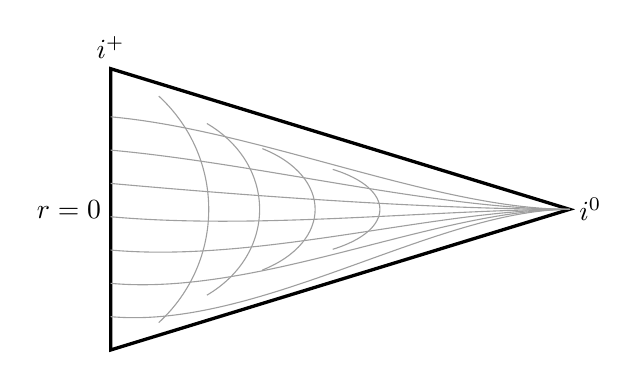
\begin{tikzpicture}[scale=0.94]
\coordinate (O) at (0,0);
\coordinate (P) at (0,3.8);
\coordinate (I) at (6.2,1.9);
\draw[very thick] (O)--(P)--(I)--cycle;
\foreach \y in {0.45,0.90,1.35,1.80,2.25,2.70,3.15} {
  \draw[gray!75] (0,\y) .. controls (2.0,\y-0.18) and (4.4,1.9) .. (I);
}
\draw[gray!75] (0.65,0.37) .. controls (1.55,1.20) and (1.55,2.60) .. (0.65,3.43);
\draw[gray!75] (1.30,0.74) .. controls (2.25,1.30) and (2.25,2.50) .. (1.30,3.06);
\draw[gray!75] (2.05,1.08) .. controls (3.00,1.46) and (3.00,2.34) .. (2.05,2.72);
\draw[gray!75] (3.00,1.36) .. controls (3.85,1.62) and (3.85,2.18) .. (3.00,2.44);
\node[left] at (0,1.9) {\(r=0\)};
\node[above] at (P) {\(i^+\)};
\node[right] at (I) {\(i^0\)};
\end{tikzpicture}
\caption{Phiên bản gọn của nêm phía trên. Các đường cong là những họ đường \(r\) không đổi và \(t\) không đổi theo nghĩa định tính, chứ không phải một lưới tọa độ chính xác.}
\label{fig:l05-flat-wedge}
\end{figure}

Các đường thế giới tại \(r\) cố định, vốn thẳng đứng trước khi compact hóa, uốn cong và dồn lại gần vô cực loại thời tương lai. Các lát \(t\) không đổi cũng tương tự mà dồn về phía vô cực không gian. Sự dồn này là một hiệu ứng tọa độ, không phải sự nén vật chất về mặt vật lý.

Quy tắc \(45^\circ\) áp dụng trực tiếp cho ánh sáng theo phương bán kính. Một tia có mômen động lượng có thể không đi qua gốc, đạt tới một khoảng cách tiếp cận gần nhất khác không, rồi quay trở ra. Ở xa gốc, chuyển động chiếu của nó trông gần như theo phương bán kính; chỉ gần điểm tiếp cận gần nhất thì quỹ đạo rút gọn trong \((t,r)\) mới cong thấy rõ. Như vậy là hoàn tất phần làm việc thứ nhất.

\section{Phần làm việc thứ hai: Schwarzschild vĩnh cửu}

Nghiệm Schwarzschild mở rộng tối đại có hai hình thoi miền ngoài, một miền lỗ đen tương lai, và một miền lỗ trắng quá khứ. Các biên lượn sóng phía trên và phía dưới của nó lần lượt là kỳ dị tương lai và kỳ dị quá khứ. Đối với một lỗ đen được tạo ra bởi sự suy sụp, phần lớn cấu trúc này sẽ sớm bị loại bỏ, nhưng miền ngoài bên phải thông thường chính là mảnh ta cần.

\begin{figure}[htbp]
\centering
\includegraphics[width=0.72\textwidth]{lecture_05_figure_03.png}
\caption{Sơ đồ Schwarzschild vĩnh cửu, với miền ngoài thông thường và lưới tọa độ sơ đồ hóa của nó ở bên phải.}
\lectureframe{00:16:55.975}
\end{figure}

\begin{figure}[htbp]
\centering
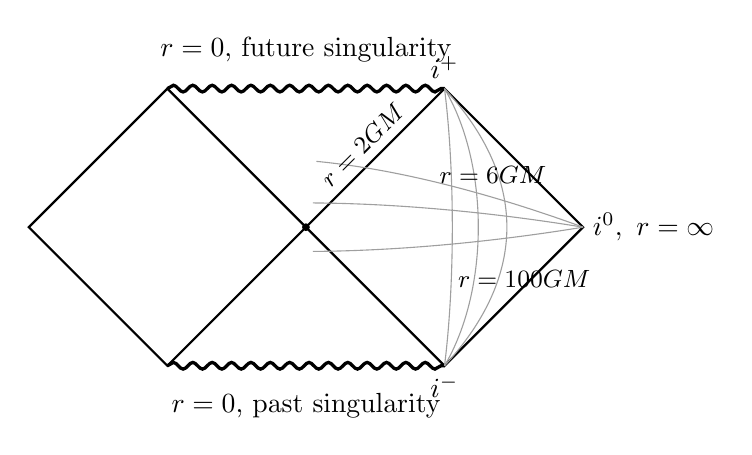
\begin{tikzpicture}[scale=0.88]
\coordinate (C) at (0,0);
\coordinate (TL) at (-2.0,2.0);
\coordinate (L) at (-4.0,0);
\coordinate (BL) at (-2.0,-2.0);
\coordinate (TR) at (2.0,2.0);
\coordinate (R) at (4.0,0);
\coordinate (BR) at (2.0,-2.0);
\draw[thick] (C)--(TL)--(L)--(BL)--(C);
\draw[thick] (C)--(TR)--(R)--(BR)--(C);
\draw[very thick,decorate,decoration={snake,amplitude=1.2pt,segment length=7pt}] (TL)--(TR);
\draw[very thick,decorate,decoration={snake,amplitude=1.2pt,segment length=7pt}] (BL)--(BR);
\draw[gray!75] (TR) .. controls (2.15,0.8) and (2.15,-0.8) .. (BR);
\draw[gray!75] (TR) .. controls (2.65,0.9) and (2.65,-0.9) .. (BR);
\draw[gray!75] (TR) .. controls (3.20,0.7) and (3.20,-0.7) .. (BR);
\draw[gray!75] (0.15,0.95) .. controls (1.5,0.82) and (2.9,0.40) .. (R);
\draw[gray!75] (0.10,0.35) .. controls (1.5,0.34) and (2.9,0.18) .. (R);
\draw[gray!75] (0.10,-0.35) .. controls (1.5,-0.34) and (2.9,-0.18) .. (R);
\fill (C) circle (1.6pt);
\node[above] at (TR) {\(i^+\)};
\node[below] at (BR) {\(i^-\)};
\node[right] at (R) {\(i^0,\ r=\infty\)};
\node[above] at (0,2.25) {\(r=0\), future singularity};
\node[below] at (0,-2.25) {\(r=0\), past singularity};
\node[rotate=45,above,font=\small] at (1.0,1.0) {\(r=2GM\)};
\node[font=\small] at (2.70,0.75) {\(r=6GM\)};
\node[font=\small] at (3.15,-0.75) {\(r=100GM\)};
\end{tikzpicture}
\caption{Miền ngoài bên phải giống nêm phẳng ở bán kính lớn. Cạnh null phía trong của nó là \(r=2GM\) khi \(c=1\); các bán kính được gắn nhãn khác chỉ là những ví dụ sơ đồ.}
\label{fig:l05-eternal-schwarzschild}
\end{figure}

Càng xa lỗ đen, miền ngoài càng giống không-thời gian phẳng đã compact hóa. Những đường như \(r=6GM\) và \(r=100GM\) tiến gần tới cách hành xử của các đường thế giới bán kính không đổi thông thường. Biên trong của miền ngoài nằm tại
\begin{equation}
r=2GM
\end{equation}
trong các đơn vị \(c=1\).

Gần tâm, phép so sánh với không-thời gian phẳng không còn đúng nữa. Một tia theo phương bán kính trong không-thời gian Minkowski đi tới \(r=0\) rồi xuất hiện trở lại ở phía vật lý đối diện. Một tia hướng tương lai ở bên trong Schwarzschild không bật lại. Nó kết thúc trên kỳ dị kiểu không gian tại \(r=0\). Chính khác biệt nhân quả ấy là điều phép dựng suy sụp phải bảo toàn.

\section{Định lý cho phép ta ghép các mảnh}

Thành phần còn thiếu trước hết xuất hiện trong hấp dẫn Newton. Đối với một phân bố khối lượng đối xứng cầu, định luật Gauss cho
\begin{equation}
\oint\mathbf g\cdot d\mathbf A=-4\pi G M_{\mathrm{enc}},
\end{equation}
và do đó
\begin{equation}
\mathbf g(r)=-\frac{G M_{\mathrm{enc}}(r)}{r^2}\,\hat{\mathbf r}.
\label{eq:l05-shell-theorem}
\end{equation}
Vật chất ở ngoài mặt cầu bán kính \(r\) không đóng góp trường tổng nào tại đó. Đối với một vỏ rỗng có tổng khối lượng \(M\),
\begin{equation}
\mathbf g=
\begin{cases}
0, & r<R_{\mathrm{shell}},\\[3pt]
-\dfrac{GM}{r^2}\hat{\mathbf r}, & r>R_{\mathrm{shell}}.
\end{cases}
\end{equation}

Định lý Birkhoff là sự thay thế tương đối tính. Mọi miền chân không đối xứng cầu đều cục bộ là một miền Schwarzschild với một tham số khối lượng không đổi. Phần trong rỗng của một vỏ cầu có tham số khối lượng bằng không và cục bộ là Minkowski; phần ngoài có tham số khối lượng \(M\) và là Schwarzschild:
\begin{equation}
\begin{aligned}
M_{\mathrm{enc}}&=0 && \text{inside the shell},\\
M_{\mathrm{enc}}&=M && \text{outside the shell}.
\end{aligned}
\label{eq:l05-birkhoff}
\end{equation}
Mệnh đề này vẫn hữu ích khi vỏ chuyển động, vì các miền chân không ở hai phía của nó vẫn giữ đối xứng cầu.

\editorialnote{Phẳng ở bên trong là một mệnh đề cục bộ. Một vỏ tĩnh có thể làm thay đổi chuẩn hóa của tọa độ thời gian bên trong mặc dù độ cong bên trong triệt tiêu. Đối với một vỏ chuyển động hoặc vỏ null, hai metric chân không phải được ghép khớp qua vỏ; phép dựng lý tưởng hóa là một ghép nối vỏ mỏng, có liên hệ chặt chẽ với hình học Vaidya đi vào. Không một điều kiện kèm theo nào trong số này làm thay đổi lập luận cắt-dán nhân quả được dùng ở đây.}

Để có một hình ảnh trong phòng thí nghiệm, hãy tưởng tượng một hình cầu phủ dày đặc các laser đồng bộ, như tại một cơ sở giam hãm quán tính cỡ lớn, tất cả cùng bắn vào trong một lúc. Trong lý tưởng hóa này không có thiết bị nào, chỉ có một vỏ ánh sáng cầu hoàn hảo. Vỏ mang năng lượng \(E\), nên tham số khối lượng bên ngoài là
\begin{equation}
M=\frac{E}{c^2},
\end{equation}
hoặc đơn giản là \(E=M\) trong đơn vị tự nhiên. Vì vỏ chuyển động với tốc độ ánh sáng, nó là một đường null đi vào trên sơ đồ rút gọn. Mỗi điểm trên đường đó biểu diễn cả một mặt sóng cầu, chứ không phải quỹ đạo của một photon.

\section{Khâu nối không-thời gian suy sụp}

Hãy bắt đầu với không-thời gian phẳng và vẽ vỏ null đi vào. Miền bên trong vỏ là đúng: định lý Birkhoff nói rằng nó phẳng. Miền bên ngoài là sai, vì hình học Schwarzschild của miền ngoài đã phải phản ánh tổng khối lượng của vỏ.

Bây giờ hãy vẽ chính vỏ ấy trong sơ đồ Schwarzschild vĩnh cửu. Ở đó miền bên ngoài vỏ là đúng. Lỗ trắng, miền ngoài thứ hai, và phần không thích hợp của miền trong lỗ đen đều sai đối với một sự suy sụp bắt đầu trong không gian trống thông thường, nên hãy xóa chúng đi.

\begin{figure}[htbp]
\centering
\includegraphics[width=0.72\textwidth]{lecture_05_figure_05.png}
\caption{Vỏ null, màu đỏ, được vẽ đè lên sơ đồ Schwarzschild trong khi phần miền ngoài đúng đang được tách ra.}
\lectureframe{00:32:00.000}
\end{figure}

Vỏ đi tới \(r=0\) trong mảnh phẳng. Trong mảnh Schwarzschild, nó đi tới điểm bắt đầu của kỳ dị tương lai. Đó là cùng một điểm cuối. Dán miền trong phẳng với miền ngoài Schwarzschild dọc theo vỏ sẽ cho không-thời gian đơn giản nhất của sự hình thành lỗ đen.

\begin{classroomqa}
\audiencequestion{Ở điểm nối phía trên bên trái, điểm cuối của phần không gian phẳng có thật sự là cùng một điểm với điểm ở phía Schwarzschild không?\lecturetimestamp{00:34:50}}
\lecturerresponse{Có. Vỏ trong không gian phẳng co lại đến \(r=0\), và kỳ dị Schwarzschild cũng ở \(r=0\). Hai điểm đang được đồng nhất có cùng ý nghĩa hình học: hai-cầu đã co lại về kích thước bằng không.}
\end{classroomqa}

\begin{figure}[htbp]
\centering
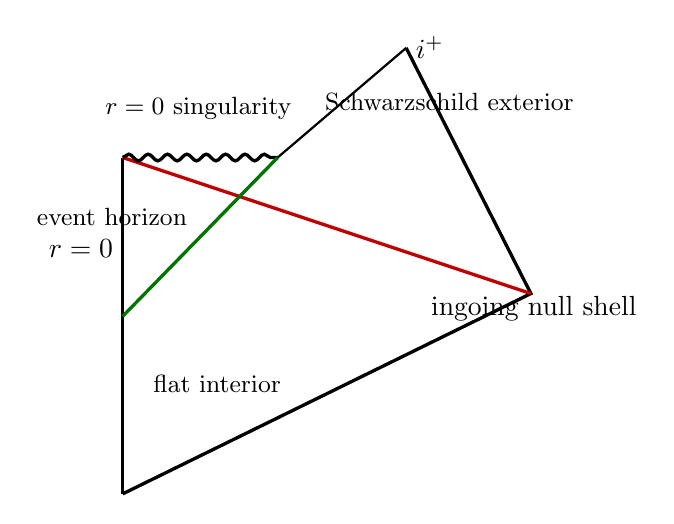
\begin{tikzpicture}[scale=0.96]
\coordinate (A) at (0,-2.8);
\coordinate (B) at (0,1.65);
\coordinate (C) at (2.05,1.65);
\coordinate (D) at (5.4,-0.15);
\coordinate (E) at (3.75,3.10);
\coordinate (H0) at (0,-0.45);
\draw[very thick] (A)--(B);
\draw[very thick] (A)--(D)--(E);
\draw[very thick,red!75!black] (D)--(B);
\draw[very thick,decorate,decoration={snake,amplitude=1.2pt,segment length=7pt}] (B)--(C);
\draw[very thick,green!45!black] (H0)--(C);
\draw[thick] (C)--(E);
\node[left] at (0,0.45) {\(r=0\)};
\node[below right] at (3.95,-0.05) {ingoing null shell};
\node[font=\small] at (1.25,-1.35) {flat interior};
\node[font=\small,anchor=west] at (2.55,2.38) {Schwarzschild exterior};
\node[above,font=\small] at (1.0,2.02) {\(r=0\) singularity};
\node[above left,font=\small] at (0.98,0.62) {event horizon};
\node[right] at (E) {\(i^+\)};
\end{tikzpicture}
\caption{Hình học suy sụp. Vỏ đỏ nối một miền trong phẳng với một miền ngoài Schwarzschild. Chân trời sự kiện màu xanh bắt đầu sớm hơn trong miền phẳng và kết thúc ở biên tương lai của miền lỗ đen.}
\label{fig:l05-collapse}
\end{figure}

Phép dựng này trả lời một câu hỏi còn bỏ ngỏ từ nghiệm vĩnh cửu. Một lỗ đen được tạo thành từ sự suy sụp không có lỗ trắng quá khứ và không có vũ trụ tiệm cận thứ hai. Nó vẫn có một kỳ dị tương lai.

\section{Chân trời là một biên toàn cục}

Nhãn cũ \(r=2GM\) dùng để nhận diện chân trời trong hình học Schwarzschild dừng, nhưng đó không phải là định nghĩa cần dùng trong một không-thời gian động.

\begin{definition}
Chân trời sự kiện tương lai là biên của tập các sự kiện có thể gửi một tín hiệu nhân quả hướng tương lai đến vô cực null tương lai.
\end{definition}

Trên sơ đồ suy sụp, hãy lần theo tia null đi ra vừa đúng không thoát được. Các tia ngay phía ngoài nó đi tới vô cực; các tia ngay phía trong nó kết thúc ở kỳ dị. Đường phân cách ấy là chân trời thực sự.

\begin{figure}[htbp]
\centering
\includegraphics[width=0.72\textwidth]{lecture_05_figure_06.png}
\caption{Phép dựng hoàn chỉnh trên bảng. Vỏ đi vào có màu đỏ còn chân trời sự kiện có màu xanh; một phần của đường xanh nằm trong miền vẫn còn phẳng ở bên dưới vỏ.}
\lectureframe{00:39:10.000}
\end{figure}

Đặc điểm gây kinh ngạc giờ đây không thể né tránh. Chân trời kéo ngược về một vùng mà lớp vỏ vẫn chưa tới. Hình học ở đó phẳng theo nghĩa cục bộ, và một người quan sát đi qua đường đó không phát hiện xung độ cong, bức tường hay tia lóe nào. Tuy nhiên, người ấy đã không còn khả năng tới vô cực, vì lớp vỏ trong tương lai sẽ khép mọi lối thoát khả dĩ. Chân trời sự kiện mang tính viễn đích đúng theo nghĩa toàn cục này: để xác định một chân trời như vậy, cần biết toàn bộ tương lai của không-thời gian.\editorialnote{Không thí nghiệm cục bộ nào có thể xác định rằng một chân trời sự kiện trơn vừa mới được vượt qua. Những khái niệm khác, chẳng hạn chân trời biểu kiến hoặc chân trời bẫy, có tính cục bộ hơn và không nhất thiết trùng với chân trời sự kiện trong quá trình sụp đổ.}

Phép ví von lỗ thoát nước tách riêng ý niệm nhân quả. Hãy hình dung một người chèo thuyền gần một lỗ thoát đã bị bịt trong một hồ nước đứng yên. Nếu nút bịt ấy cứ ở nguyên mãi mãi, người chèo thuyền có thể rời đi. Nếu chắc chắn sẽ có người rút nó ra, thì dòng chảy về sau có thể khiến việc thoát ra trở nên bất khả dù hiện vẫn chưa có nước nào chuyển động. Một thác Niagara bị đóng băng cũng nêu đúng ý đó: nước yên lặng không bảo đảm một lối thoát an toàn trong tương lai.

\begin{classroomqa}
\audiencequestion{Có phải nút bịt bị rút ra vì lớp vỏ cầu ánh sáng trở nên ngày càng tập trung hơn không?\lecturetimestamp{00:43:13}}
\lecturerresponse{Sự tập trung ấy tạo ra lỗ đen, nhưng câu chuyện lỗ thoát nước đang được dùng cho một mục đích hẹp hơn: người ta đã có thể ở bên kia điểm không thể quay lại trước cả khi bất cứ điều gì kịch tính nào xảy ra tại chỗ.}
\end{classroomqa}

\subsection{Một chân trời được tạo bởi các mặt cầu lớn dần}

Mỗi điểm trên chân trời rút gọn biểu diễn một \(S^2\). Ở điểm đầu tiên của chân trời, mặt cầu ấy có diện tích bằng không. Đi lên dọc theo chân trời, mặt cầu lớn dần cho đến khi bán kính diện tích của nó đạt tới
\begin{equation}
R_s=\frac{2GM}{c^2}.
\end{equation}
Nó giữ nguyên kích thước đó đối với một lỗ đen tĩnh và lại lớn lên nếu có thêm năng lượng rơi vào.

\editorialnote{Trong giản đồ sụp đổ cầu đối xứng lý tưởng hóa, các đường sinh của chân trời gặp nhau tại một điểm hình thành, hay một nếp gấp, trên \(r=0\). Chính mặt 2-cầu giới hạn này có diện tích bằng không; không nên hiểu phát biểu đó là một chân trời Schwarzschild hữu hạn đột ngột co lại thành một điểm.}

\subsection{Những gì người quan sát ở xa có thể tái dựng}

Phần thảo luận dài tiếp theo tách một người quan sát đã ở bên trong chân trời toàn cục ra khỏi lịch sử đã đưa người ấy tới đó.

\begin{classroomqa}
\audiencequestion{Địa vị của người bị mắc kẹt trước khi lớp vỏ tới là gì? Theo quan điểm của người quan sát ở xa thì người đó có ở ngoài chân trời không?\lecturetimestamp{00:44:03}}
\lecturerresponse{Không. Một khi đường thế giới đã nằm phía sau chân trời sự kiện, tương lai của nó đi tới kỳ dị và không có tín hiệu mới nào từ nó tới được người quan sát ở xa. Tuy nhiên, người đó không bắt đầu tồn tại ở đó. Những hạt trước đó, tổ tiên, hoặc dạng năng lượng tiền thân khác đã đi vào từ một vùng còn nhìn thấy được.}
\end{classroomqa}

Vì thế, người quan sát ở xa có thể thấy vật chất tiền thân tiến gần chân trời mà không bao giờ nhận được tín hiệu nào từ phía bên kia nó. Không có mâu thuẫn nào trong việc nhìn xuyên qua lớp vỏ đang đi vào: nó được tạo bởi ánh sáng, và người quan sát cũng có thể nhìn thấy chính lớp vỏ ấy rồi suy ra rằng một lỗ đen đã hình thành.

\begin{classroomqa}
\audiencequestion{Đường ngắm có đi xuyên qua lớp vỏ đang co sụp không, và người quan sát bên ngoài vẫn có thể biết rằng lỗ đen đã hình thành chứ?\lecturetimestamp{00:46:51}}
\lecturerresponse{Có. Người quan sát nhìn thấy lớp vỏ đi vào và có thể nhận ánh sáng có đường đi cắt qua nó trong khi ánh sáng ấy vẫn còn thoát ra được. Điều trông có vẻ lạ là vật chất tiền thân tiến tới chân trời vừa được xác định ngay cả trước khi lớp vỏ chạm tới tâm.}
\end{classroomqa}

\begin{classroomqa}
\audiencequestion{Điều này có tiếp tục khẳng định quy tắc rằng, nhìn từ bên ngoài, vật chất trông như đã bị nén lên chân trời không?\lecturetimestamp{00:47:49}}
\lecturerresponse{Có. Trong mô tả từ bên ngoài, nó vẫn gắn với chân trời, ngày càng bị đỏ dịch mạnh hơn, cho đến khi quá trình lượng tử về sau là sự bốc hơi lỗ đen làm thay đổi câu chuyện.}
\end{classroomqa}

Mô tả từ bên ngoài này dẫn sang chủ đề tiếp theo. Nếu thông tin dường như bị dán lên một bề mặt hai chiều, thì việc entropy lỗ đen tỉ lệ theo diện tích của bề mặt đó sẽ bớt gây ngạc nhiên hơn.

\section{Entropy và nhiệt độ quan sát từ vô cực}

Gần một chân trời lớn, ta có thể thay bề mặt cầu bằng một mặt phẳng cục bộ, cũng như ta dùng xấp xỉ Trái Đất phẳng trong một phòng thí nghiệm nhỏ. Khi đó, hai sự kiện từ phần thảo luận trước được ghép lại với nhau:
\begin{equation}
\begin{aligned}
S_{\mathrm{BH}}&\propto A_H,\\
\Delta A_H&\sim \ell_P^2
\quad\text{per added bit, schematically}.
\end{aligned}
\end{equation}
Quy tắc ghi nhớ một bit trên mỗi diện tích Planck diễn đạt định luật diện tích; đó không phải là một suy dẫn vi mô.

Nhiệt độ Hawking đo ở xa một lỗ đen Schwarzschild là
\begin{equation}
T_H=\frac{\hbar c^3}{8\pi GMk_B}.
\label{eq:l05-hawking}
\end{equation}
Với \(R_s=2GM/c^2\),
\begin{equation}
T_H=\frac{\hbar c}{4\pi k_B R_s}.
\label{eq:l05-hawking-radius}
\end{equation}
Vì vậy, lỗ đen càng lớn thì càng lạnh.

\begin{classroomqa}
\audiencequestion{Nhiệt độ có thể phụ thuộc vào vị trí không?\lecturetimestamp{00:52:43}}
\lecturerresponse{Trong cách nói thông thường thì rõ ràng là có: New York và Stanford không nhất thiết có cùng nhiệt độ. Câu hỏi sắc nét hơn liên quan đến một hệ ở cân bằng nhiệt hấp dẫn. Khi đó, số đo nhiệt kế cục bộ có thể thay đổi theo độ cao dù nhiệt độ cân bằng đã tính đến đỏ dịch là hằng số.}
\end{classroomqa}

Nhiệt độ được đọc thông qua các năng lượng động học cục bộ. Trong một khí quyển loãng phía trên một Trái Đất được nung nóng, các phân tử mất năng lượng động học khi đi lên và thu thêm khi đi xuống. Photon bị đỏ dịch khi đi lên và bị lam dịch khi đi xuống. Vì vậy, một nhiệt kế thấp và một nhiệt kế cao không nhất thiết chỉ cùng một thang năng lượng cục bộ.

Đối với một không-thời gian tĩnh, hệ thức cân bằng là
\begin{equation}
T_{\mathrm{loc}}(r)\sqrt{-g_{tt}(r)}=T_\infty,
\label{eq:l05-tolman}
\end{equation}
đó là định luật Tolman. Nhiệt độ Hawking trong Phương trình~\eqref{eq:l05-hawking} là \(T_\infty\), tức số đo được chuẩn hóa tại vô cực.

\section{Khí quyển tĩnh nóng gần chân trời}

Gọi \(\rho\) là khoảng cách riêng đo ra ngoài từ chân trời. Gần một chân trời Schwarzschild lớn, Phương trình~\eqref{eq:l05-tolman} trở thành
\begin{equation}
k_B T_{\mathrm{loc}}(\rho)
\simeq\frac{\hbar c}{2\pi\rho},
\label{eq:l05-local-temperature-si}
\end{equation}
hoặc, trong đơn vị \(c=\hbar=k_B=1\),
\begin{equation}
T_{\mathrm{loc}}(\rho)=\frac{1}{2\pi\rho}.
\label{eq:l05-local-temperature}
\end{equation}

\begin{figure}[htbp]
\centering
\includegraphics[width=0.72\textwidth]{lecture_05_figure_07.png}
\caption{Nhiệt độ Hawking tiệm cận và nhiệt độ cục bộ gần chân trời \(T(\rho)=1/(2\pi\rho)\) trên bảng.}
\lectureframe{01:02:40.000}
\end{figure}

Một nhiệt kế nhỏ xíu được giữ bằng cáp tại \(\rho\) cố định sẽ cho biết nhiệt độ tăng dần khi nó được hạ xuống. Một nguyên tử được giữ trong khí quyển tĩnh đó sẽ bị kích thích, rồi bị ion hóa, rồi bị phá vỡ; ở những năng lượng cục bộ còn lớn hơn nữa, ngay cả hạt nhân và hadron cũng không còn giữ được tính toàn vẹn. Hạ một người xuống bằng chân trước cho ta một chẩn đoán dễ nhớ: nóng chân.

Từ \emph{được giữ} là thiết yếu. Sự phân kỳ này gắn với một đầu dò được giữ đứng yên nhờ gia tốc. Nó mô tả khí quyển nhiệt khi được đỏ dịch theo thời gian bên ngoài. Một đầu dò rơi tự do đi theo một quỹ đạo khác và, đối với một lỗ đen đủ lớn trong một trạng thái lượng tử chính quy, không nhất thiết gặp một bể nhiệt phân kỳ tại chân trời.\editorialnote{Sự phân biệt này tách nhiệt độ Tolman và nhiệt độ gia tốc mà các người quan sát tĩnh nhìn thấy khỏi trải nghiệm cục bộ bình thường của một người quan sát rơi tự do. Bài giảng cố ý biến sự tương phản đó thành một câu đố thao tác được, thay vì giải quyết nó chỉ bằng thuật ngữ.}

Ngưỡng ion hóa làm cho sự xung đột trở nên cụ thể.

\begin{classroomqa}
\audiencequestion{Cần bao nhiêu năng lượng để ion hóa hydro?\lecturetimestamp{01:06:53}}
\lecturerresponse{Cả lớp nêu \(13\) electron volt, qua đó xác định đúng \(13.6\,\mathrm{eV}\) là năng lượng ion hóa từ trạng thái cơ bản. Ước lượng đi kèm cỡ vài nghìn kelvin là quá nhỏ, nhưng đối với lập luận này chỉ cần sự tồn tại của một ngưỡng hữu hạn.}
\end{classroomqa}

Thật vậy,
\begin{equation}
\frac{13.6\,\mathrm{eV}}{k_B}\simeq1.58\times10^5\,\mathrm{K}.
\end{equation}
Vì thế tồn tại một khoảng cách riêng nhỏ nào đó \(\rho_{\mathrm{ion}}\) mà tại đó nhiệt độ tĩnh đạt tới thang ion hóa. Một phép ngoại suy tĩnh nói rằng nguyên tử lẽ ra đã bị ion hóa ở đó, bên ngoài chân trời. Trái lại, một nguyên tử rơi tự do không chờ đợi một bức tường cục bộ nào và có thể vượt qua chân trời trong thời gian riêng hữu hạn. Liệu một người quan sát bên ngoài có thể thực hiện một thí nghiệm quyết định giữa hai mô tả này không?

\section{Kính hiển vi Heisenberg}

Trước khi áp dụng câu hỏi đó cho lỗ đen, hãy nhớ lại kính hiển vi photon. Để định vị một hạt với độ phân giải \(\Delta x\), bước sóng đầu dò phải thỏa
\begin{equation}
\lambda\lesssim\Delta x.
\end{equation}
Khi đó, một photon mang động lượng ít nhất là
\begin{equation}
p_\gamma\gtrsim\frac{\hbar}{\Delta x}.
\label{eq:l05-microscope}
\end{equation}
Sự tán xạ photon ấy tạo ra một độ giật lùi cùng bậc. Nếu trước hết đo vị trí rồi kiểm tra vận tốc ngay lập tức, phép đo thứ hai sẽ thấy một trạng thái đã bị phép đo thứ nhất làm thay đổi. Thí nghiệm tạo ra chính điều kiện mà nó định loại trừ.

\begin{figure}[htbp]
\centering
\includegraphics[width=0.70\textwidth]{lecture_05_figure_08.png}
\caption{Kính hiển vi cho ước lượng \(\Delta x\gtrsim\lambda\) và \(p_\gamma\gtrsim\hbar/\Delta x\).}
\lectureframe{01:11:50.000}
\end{figure}

Đây không chỉ đơn thuần là một giới hạn của quang học cổ điển. Sóng cổ điển có thể được làm yếu tùy ý; cơ học lượng tử đòi hỏi ít nhất một lượng tử trong một sự kiện phát hiện thành công. Vì vậy, việc cải thiện độ phân giải không gian buộc phải có một sự truyền động lượng hữu hạn.

\section{Thí nghiệm gần chân trời}

Bây giờ hãy để một nguyên tử rơi qua lớp bắt đầu tại \(\rho_{\mathrm{ion}}\). So với khung tĩnh, nó đang chuyển động vào trong với tốc độ gần \(c\), nên khoảng thời gian sẵn có trước khi vượt qua chân trời có bậc
\begin{equation}
\Delta\tau\sim\frac{\rho_{\mathrm{ion}}}{c}.
\label{eq:l05-fall-time}
\end{equation}
Sau khi vượt qua, không thể gửi kết quả nào trở lại bên ngoài. Phép đo phải phân biệt một nguyên tử còn nguyên vẹn với một nguyên tử đã bị ion hóa trong khoảng ngắn này.

Để phân giải nguyên tử trong lớp đó cần
\begin{equation}
\lambda\lesssim\rho_{\mathrm{ion}}.
\end{equation}
Do đó năng lượng đầu dò bị chặn dưới bởi
\begin{equation}
E_\gamma=cp_\gamma
\gtrsim\frac{\hbar c}{\rho_{\mathrm{ion}}}.
\label{eq:l05-probe-energy}
\end{equation}
Ngoài thừa số \(2\pi\), đây là cùng một thang như Phương trình~\eqref{eq:l05-local-temperature-si}:
\begin{equation}
E_\gamma\gtrsim2\pi k_B T_{\mathrm{loc}}(\rho_{\mathrm{ion}}).
\label{eq:l05-probe-temperature}
\end{equation}
Photon đủ năng lượng để phân giải sự kiện cũng đồng thời đủ năng lượng để ion hóa nguyên tử.

\begin{figure}[htbp]
\centering
\includegraphics[width=0.72\textwidth]{lecture_05_figure_09.png}
\caption{Ước lượng gần chân trời trên bảng: \(\lambda<\rho\) buộc năng lượng đầu dò cục bộ phải có bậc \(\hbar c/\rho\).}
\lectureframe{01:18:30.000}
\end{figure}

\begin{classroomqa}
\audiencequestion{Liệu photon năng lượng cao đó có ion hóa nguyên tử ngay cả trong hệ quy chiếu rơi tự do của nó không?\lecturetimestamp{01:19:07}}
\lecturerresponse{Có. Nguyên tử bị đánh trúng bởi một lượng tử năng lượng cao có thật và bị giật lùi hoặc bị ion hóa trong chính hệ quy chiếu cục bộ của nó. Phép đo không bộc lộ một sự rơi không bị nhiễu; nó thay thế sự rơi ấy bằng một sự rơi đã bị nhiễu.}
\end{classroomqa}

\begin{classroomqa}
\audiencequestion{Nếu nguyên tử cứ đơn giản rơi xuống và không ai thực hiện thí nghiệm thì sao?\lecturetimestamp{01:19:39}}
\lecturerresponse{Khi đó, nhiễu động riêng này không có mặt. Nếu một người quan sát bên ngoài thực sự tiến hành thí nghiệm độ phân giải cao, thì nguyên tử sẽ gặp nguy. Lập luận này liên quan đến điều gì có thể được kiểm chứng từ bên ngoài, chứ không phải là một chứng minh rằng một vật rơi vào không bị đo sẽ bị thiêu cháy.}
\end{classroomqa}

\subsection{Nhiệt kế hay bộ phát tín hiệu có thể làm tốt hơn không?}

Di chuyển thiết bị không loại bỏ được vấn đề thông tin.

\begin{classroomqa}
\audiencequestion{Liệu ta có thể đo ở xa hơn, suy ra gradien, hoặc để một nhiệt kế rơi tự do ghi lại nhiệt độ rồi thu hồi nó sau đó không?\lecturetimestamp{01:19:51}}
\lecturerresponse{Để biết bản ghi gần chân trời, phải có một cái gì đó tương tác với nhiệt kế và mang thông tin trở lại dưới dạng các lượng tử. Quay đầu nhiệt kế lại đòi hỏi gia tốc dữ dội, còn đọc nó từ xa thì đòi hỏi phát xạ hoặc tán xạ. Cả hai con đường đều làm thay đổi chính hệ vật lý mà ta muốn kiểm tra lịch sử không bị nhiễu của nó.}
\end{classroomqa}

\begin{classroomqa}
\audiencequestion{Năng lượng đầu dò cao cần cho độ phân giải nhỏ có phải cũng chính là khó khăn khi đưa tín hiệu phản xạ của phép quan sát ra khỏi vùng gần chân trời không?\lecturetimestamp{01:21:51}}
\lecturerresponse{Chúng là hai mặt của cùng một thang đã đỏ dịch. Photon có thể có năng lượng thấp khi cuối cùng nó tới vô cực vì nó mất năng lượng khi leo ra ngoài, nhưng nó phải có tần số cục bộ cao tại nơi nó phân giải nguyên tử.}
\end{classroomqa}

\editorialnote{Một photon phát ra ngay bên ngoài chân trời không nhất thiết phải mang năng lượng lớn chỉ để thoát ra. Yêu cầu quyết định ở đây là nó phải mã hóa sự kiện trong một thời gian riêng và một khoảng cách riêng cỡ \(\rho\); khi đó, dịch đỏ hấp dẫn liên hệ tần số cục bộ lớn ấy với một tần số tiệm cận nhỏ hơn nhiều.}

\begin{classroomqa}
\audiencequestion{Liệu vật thể có thể tự phát ra thông tin thay vì bị một photon bên ngoài chiếu vào không?\lecturetimestamp{01:22:51}}
\lecturerresponse{Có, nhưng sự phát xạ cục bộ đó vẫn cần băng thông cần thiết để nhận diện điều gì đã xảy ra trong khoảng thời gian ngắn ấy. Sự phát xạ cũng làm vật thể bị giật lùi. Việc thay ánh sáng phản xạ bằng một bộ phát không cho ta một bản ghi nào mà không phải trả giá.}
\end{classroomqa}

\begin{classroomqa}
\audiencequestion{Nguyên tử đang rơi có một hướng ưu tiên. Động năng có hướng của nó có đang bị gọi là nhiệt độ không?\lecturetimestamp{01:23:10}}
\lecturerresponse{Không. Ném một quả bóng chày không làm quả bóng chày nóng lên. Năng lượng rơi vào của chuyển động khối và sự khuấy động nhiệt là hai thứ khác nhau. Nhiệt độ trong lập luận thuộc về môi trường bức xạ tĩnh xung quanh, chứ không thuộc về chuyển động của tâm khối lượng của nguyên tử.}
\end{classroomqa}

\begin{classroomqa}
\audiencequestion{Liệu một phòng thí nghiệm cùng rơi có thể dùng từ trường để kiểm tra xem nguyên tử có bị ion hóa hay không?\lecturetimestamp{01:23:50}}
\lecturerresponse{Một phòng thí nghiệm có thể thực hiện một phép kiểm tra cục bộ. Khó khăn là truyền kết quả của nó trở lại bên ngoài trước khi vượt qua. Việc truyền thông tin đó một lần nữa đòi hỏi một tương tác và các lượng tử phát ra ngoài với độ phân giải cục bộ cần thiết.}
\end{classroomqa}

\begin{classroomqa}
\audiencequestion{Liệu một bộ phát được tích hợp vào nhiệt kế có cần nhiều năng lượng cục bộ đến mức phá hủy thiết bị không?\lecturetimestamp{01:24:57}}
\lecturerresponse{Đó cũng chính là cùng một trở ngại, nhưng dưới dạng kỹ thuật. Ở đủ gần chân trời, năng lượng tín hiệu cần thiết trên thang cục bộ thích hợp có thể so sánh với thang nhiệt đang được kiểm tra.}
\end{classroomqa}

\begin{classroomqa}
\audiencequestion{Phải chăng vùng nhiệt độ cao mỏng đến mức không có thời gian để thực hiện phép đo một cách thong thả?\lecturetimestamp{01:25:15}}
\lecturerresponse{Đúng vậy. Độ dày riêng của nó có bậc \(\rho\), và thời gian đi qua có bậc \(\rho/c\). Có thể mô tả giới hạn này như độ phân giải không gian hoặc băng thông thời gian; theo cách mô tả nào thì nó cũng đòi hỏi xung lượng hoặc năng lượng cục bộ lớn.}
\end{classroomqa}

Ước lượng thời gian–băng thông tương ứng là
\begin{equation}
\Delta E\,\Delta\tau\gtrsim\hbar.
\end{equation}
Ở đây, hệ thức này nên được hiểu như một cận về độ phân giải theo nghĩa Fourier hay thao tác, chứ không phải như một hệ thức bất định toán tử có cùng địa vị với \(\Delta x\,\Delta p\geq\hbar/2\). Bài giảng viện dẫn bất định thời gian–năng lượng theo lối trực giác; Phương trình~\eqref{eq:l05-probe-energy}, được suy ra từ độ phân giải không gian, là phần vững chắc hơn của lập luận.

\begin{classroomqa}
\audiencequestion{Liệu có thể dùng các đầu dò năng lượng thấp hơn, độ phân giải thấp hơn trên nhiều nguyên tử và khôi phục câu trả lời bằng thống kê không?\lecturetimestamp{01:26:26}}
\lecturerresponse{Đây là một câu hỏi hợp lý, và trong lớp học nó được để ngỏ. Mỗi nguyên tử chỉ cung cấp một lần đi qua, và bất kỳ tín hiệu nào được khôi phục vẫn phải mang đủ thông tin để nhận diện sự kiện ngắn ngủi gần chân trời ấy. Bài giảng viện đến nguyên lý bất định nhưng không đưa ra một chứng minh bất khả hoàn chỉnh về mặt thống kê.}
\end{classroomqa}

\enlargethispage{2\baselineskip}
\section{Điều đã và chưa được xác lập}

Lập luận này không dự đoán rằng một người rơi tự do nhất thiết phải cảm thấy nhiệt độ tĩnh phân kỳ.

\begin{classroomqa}
\audiencequestion{Có phải ta đang nói rằng ta có thể dự đoán người đang rơi sẽ không cảm thấy nhiệt độ ấy không?\lecturetimestamp{01:27:38}}
\lecturerresponse{Không. Kết quả hẹp hơn thế: một thí nghiệm từ bên ngoài được thiết kế để xác nhận rằng nguyên tử đã không trải qua nhiễu loạn nhiệt độ cao lại tạo ra một nhiễu loạn cùng thang. Đó là tất cả những gì phân tích thao tác này xác lập.}
\end{classroomqa}

Vì vậy, kết luận không phải là một định lý firewall, cũng không phải là một chứng minh rằng vật rơi vào bị thiêu đốt, cũng không phải là một chứng minh rằng không có gì xảy ra. Nó là một giới hạn đối với sự kiểm chứng từ bên ngoài: \emph{việc phân giải sự kiện gần chân trời không bị nhiễu đòi hỏi một đầu dò làm nhiễu nó}.
Nếu thí nghiệm được thực hiện, các lượng tử của nó tạo ra hiệu ứng mà nó nhằm kiểm tra. Nếu không thực hiện, riêng lập luận này không gán thêm sự kiện nào có thể tiếp cận được bằng thực nghiệm. Sự so sánh với thí nghiệm hai khe là có chủ ý: việc hỏi hạt đã đi qua khe nào khi không có phép đo đường đi, và việc hỏi một thiết bị bên ngoài xác nhận điều gì khi không có tương tác, đều là những nỗ lực gán một câu trả lời theo nghĩa thao tác ở nơi không thể thu được bằng chứng được đề xuất.
